\label{Auswertung}

Sie befinden sich im Hauptmenü, möchten die Mikro-SD-Karte entfernen und die letzte Messung auslesen.
\begin{itemize}
	\item Wählen und bestätigen Sie im Hauptmenü den Punkt <Read last Measurement>. 
\end{itemize}

\begin{figure}[!hbt]
	\centering
	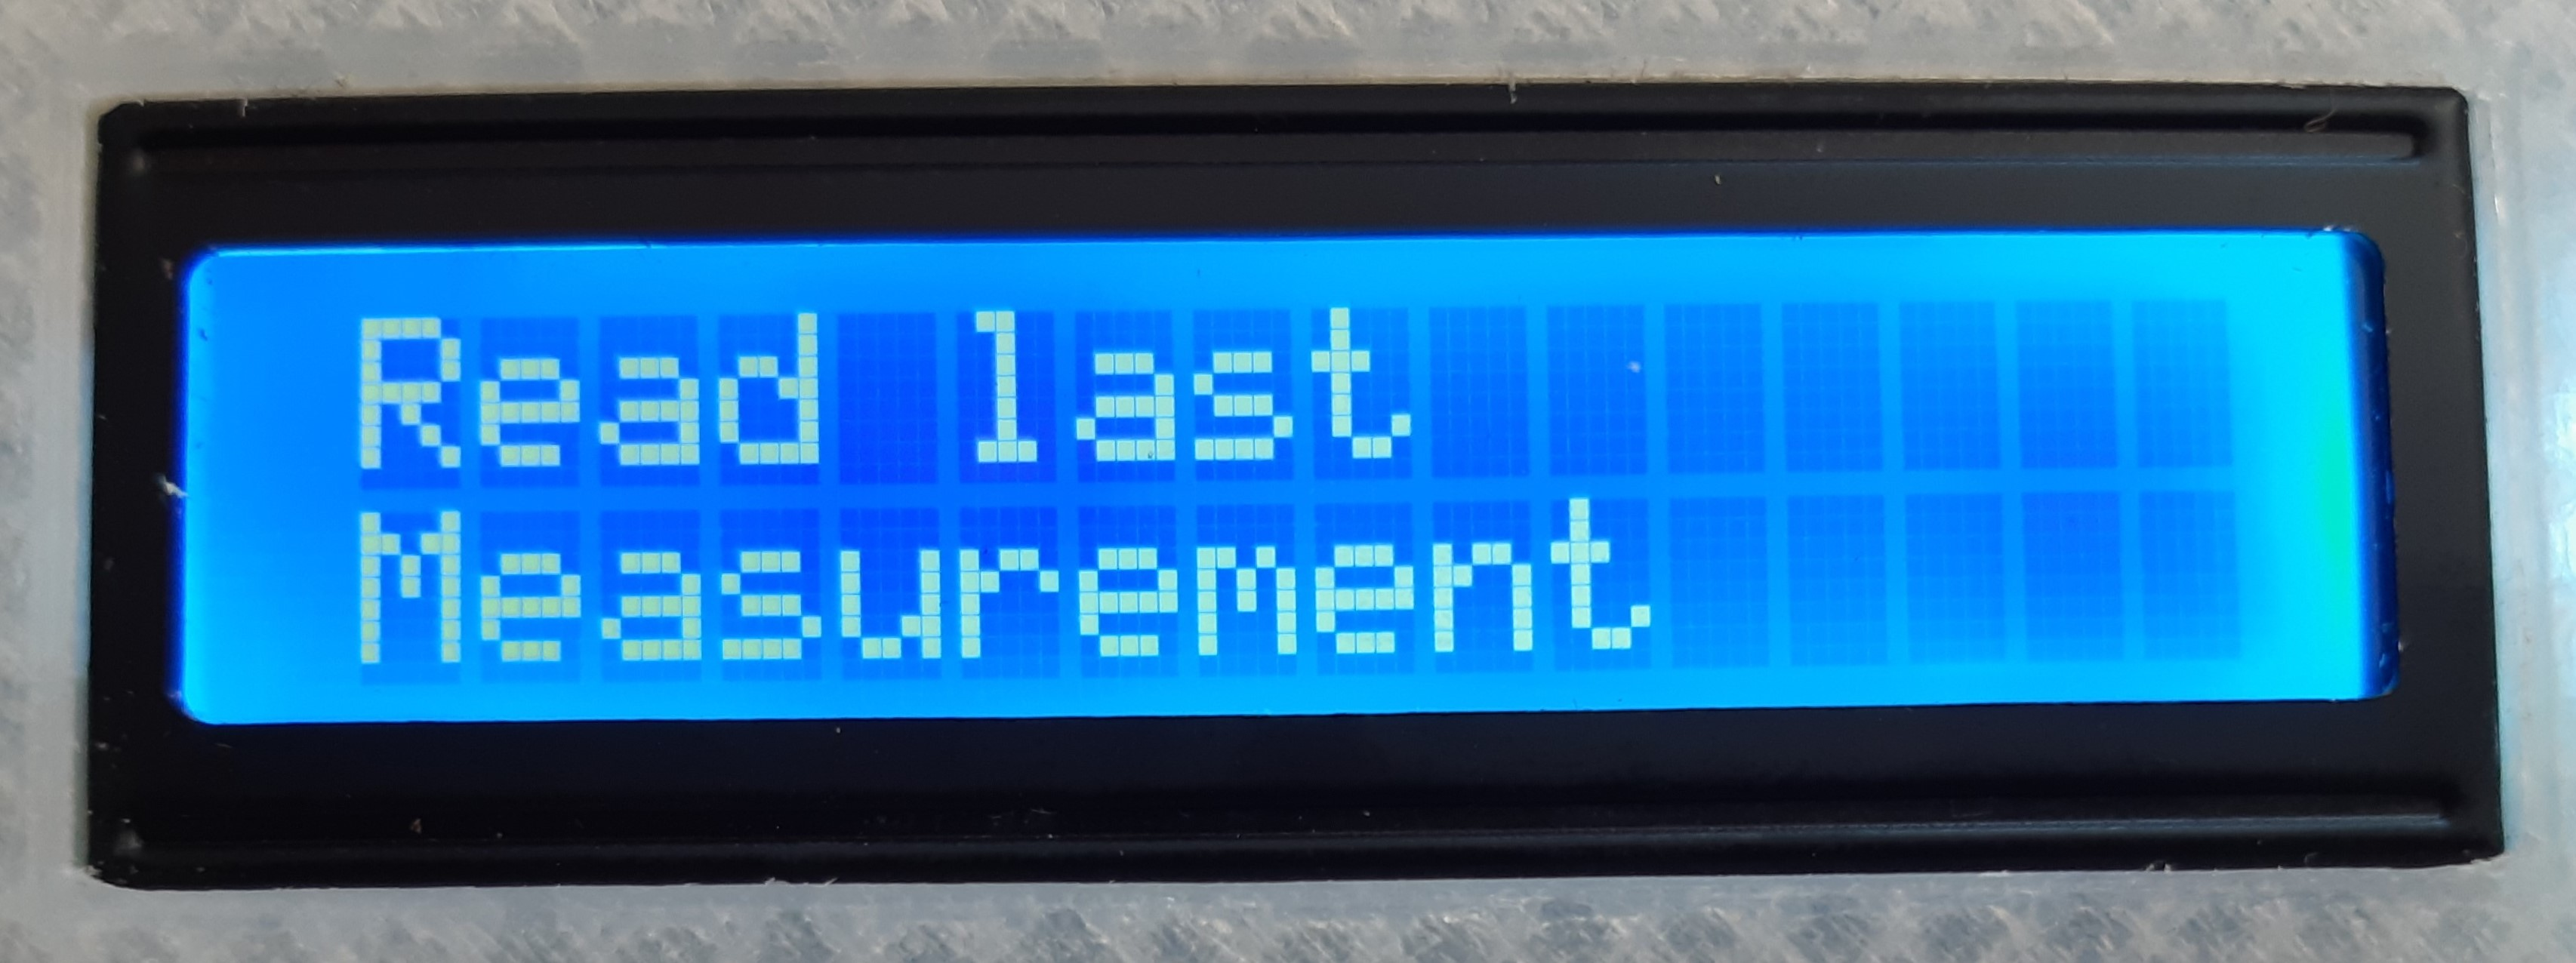
\includegraphics[width=0.3\linewidth]{Images/ReadLastMeasurement2}
	\footnotesize \\Quelle: eigene Aufnahme
	\caption{Hauptmenü: <Read last Measurement>}
	\label{fig:Readlast}
\end{figure}

Anschließend leuchten die \ac{LED}s in den Farben grün, gelb und rot auf. Sie können nun die Mikro-SD-Karte entfernen und ihre Messung analysieren. Lesen Sie dazu die Mikro-SD-Karte mit ihrem Computer aus.

\begin{figure}[!hbt]
	\centering
	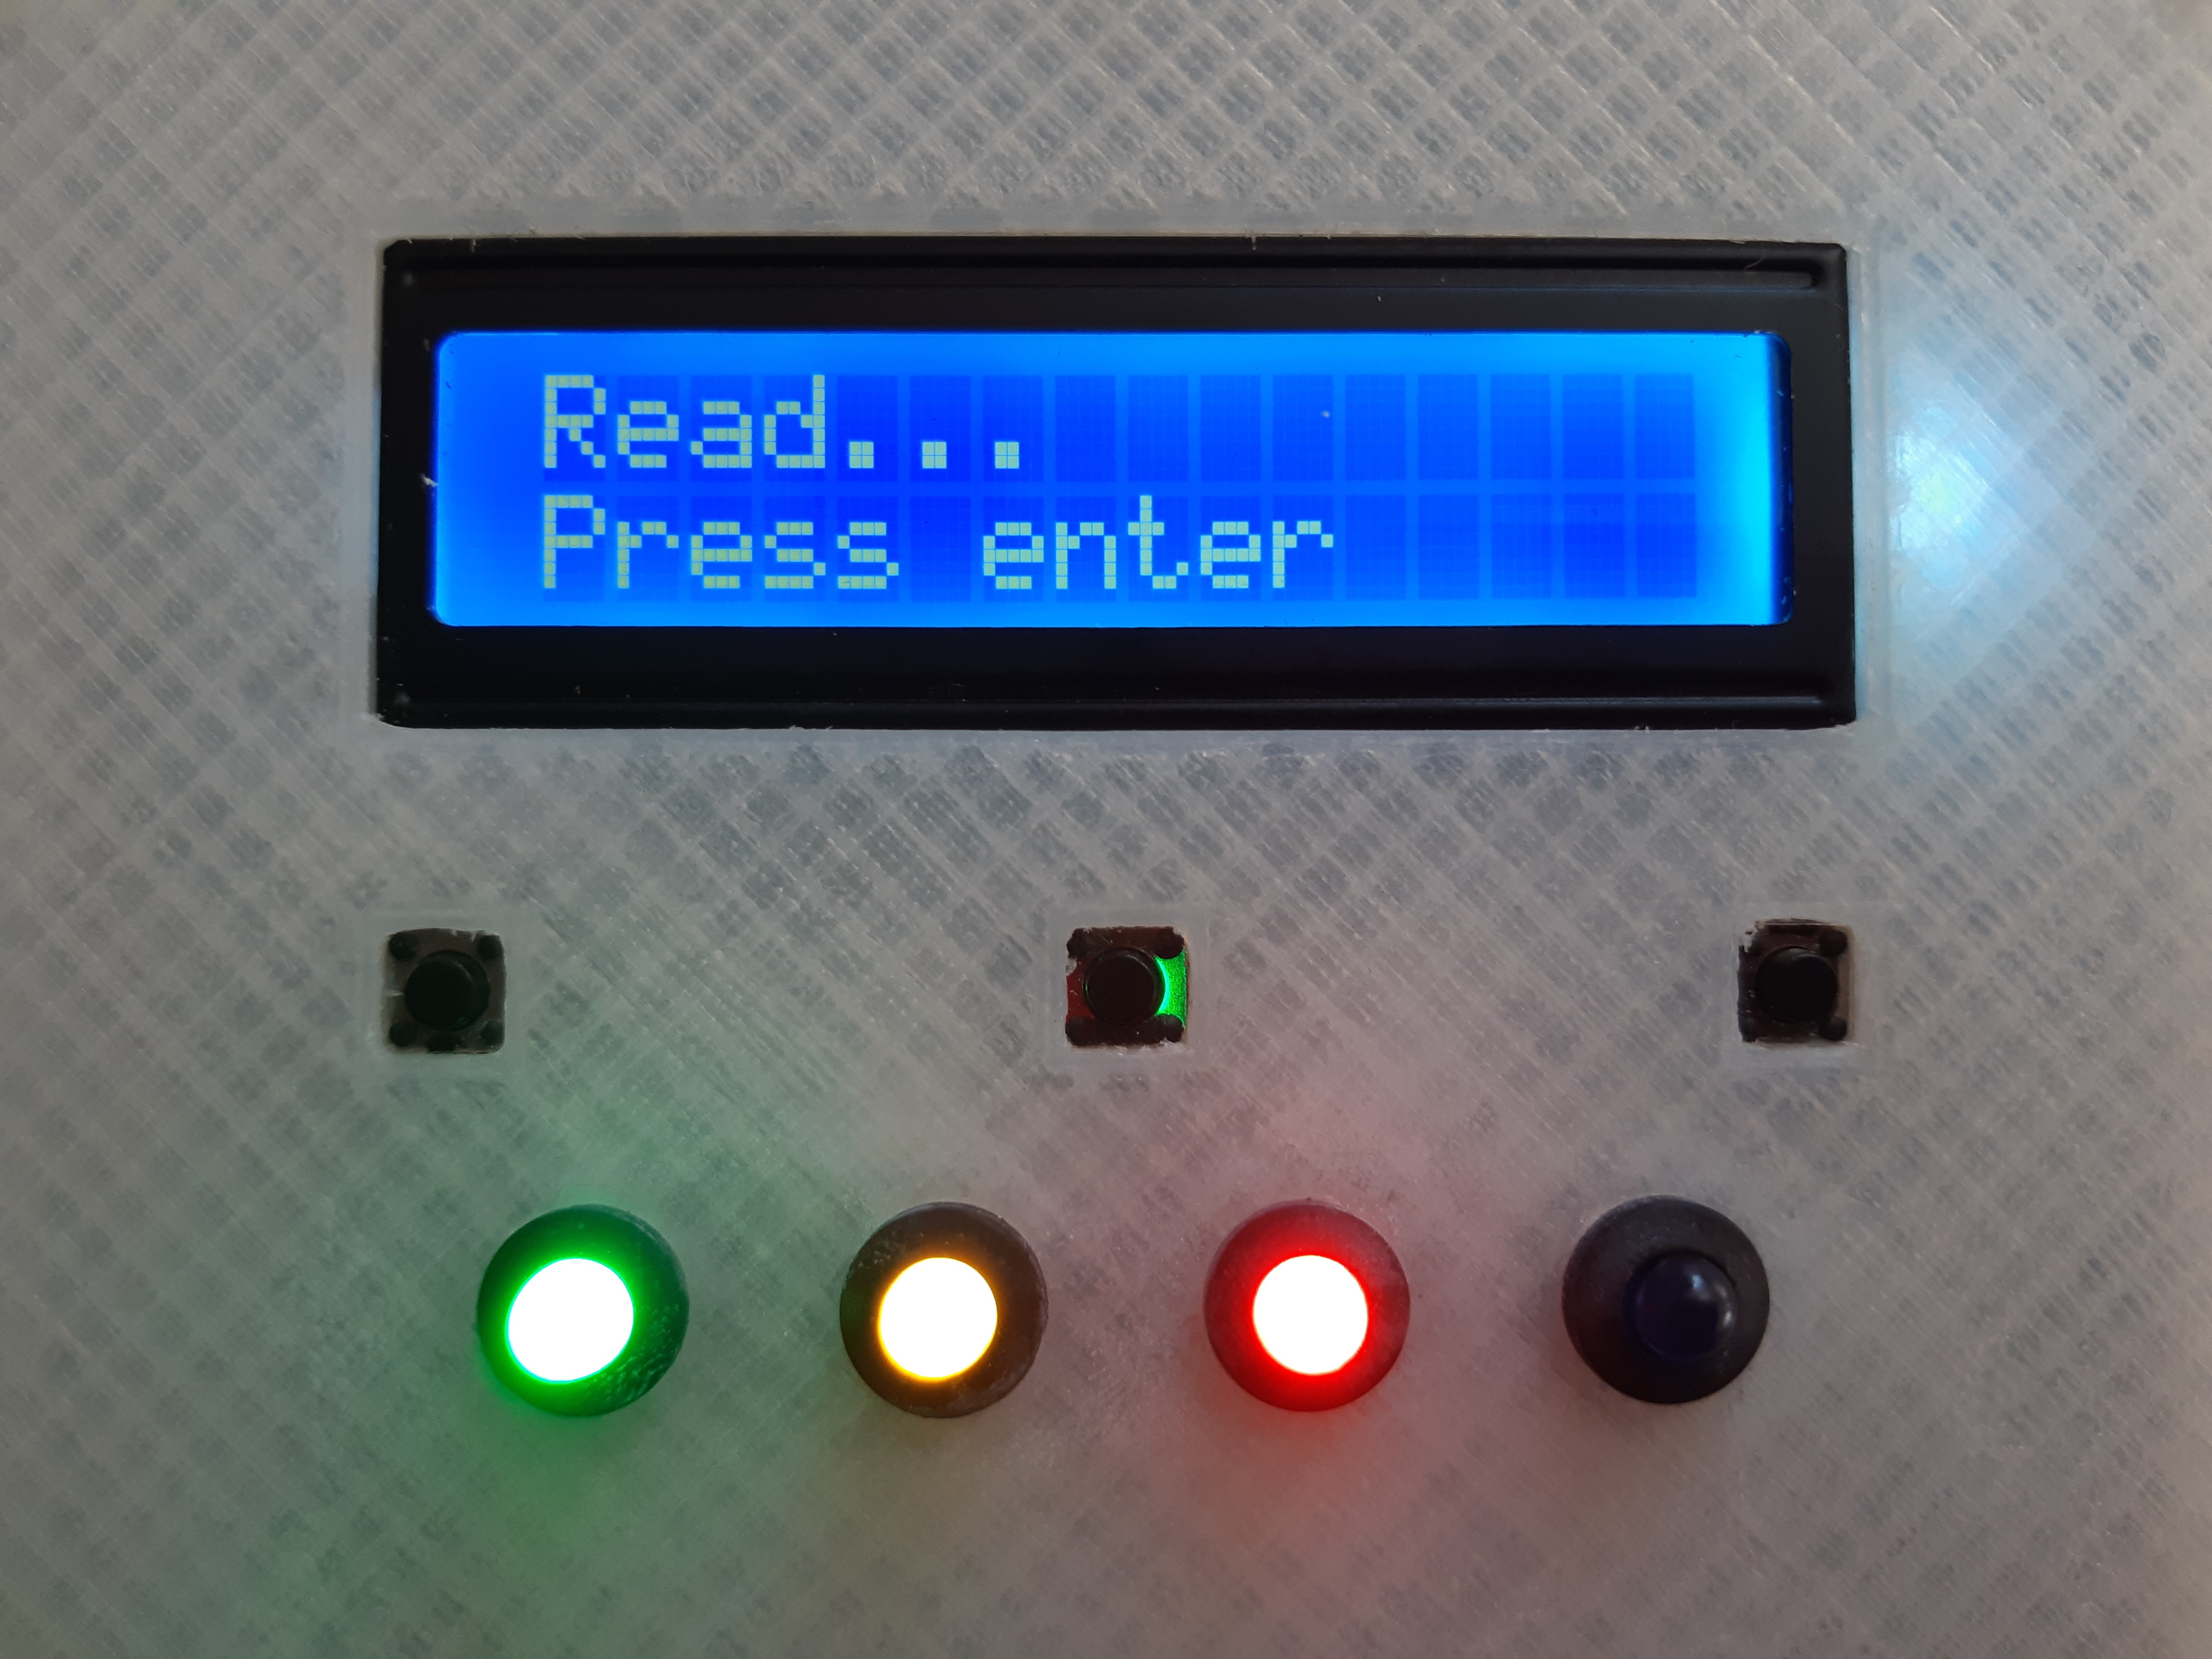
\includegraphics[width=0.3\linewidth]{Images/Read}
	\footnotesize \\Quelle: eigene Aufnahme
	\caption{Auslesemodus}
	\label{fig:Read}
\end{figure}
 
\begin{itemize}
	\item Öffnen Sie die Datei <MEASURE.txt> mit Excel.
	\item Makieren Sie die angezeigten Werte und wählen Sie ein passendes Diagramm aus.
\end{itemize}
Ihre Messung wird nun als Funktion über die Anzahl der Messungen dargestellt. Bestätigen Sie nach dem Wiedereinfügen der SD-Karte mit dem mittleren Taster. Sie befinden sich nun wieder im Hauptmenü.
